\documentclass[a4paper,10pt]{scrartcl}
\usepackage[utf8x]{inputenc}
\usepackage{color}
\usepackage{hyperref}
\usepackage{listings}
\usepackage{graphicx}
\usepackage{tikz}
\usepackage{fancyhdr}
\usetikzlibrary{arrows,shapes,petri,shadows}
\usepackage{lastpage}


%opening
\title{LpzRobots and GoRobotos}
\subtitle{An installation manual}
\author{Frank Hesse, Christoph Rauterberg}

\begin{document}
 \tikzstyle{vertex}=[circle,fill=black!25,minimum size=20pt,inner sep=0pt]
 \tikzstyle{blue vertex} = [vertex, fill=blue!30]
 \tikzstyle{green vertex} = [vertex, fill=green!30]
 \tikzstyle{red vertex} = [vertex, fill=red!30]
 \tikzstyle{edge} = [draw,thick,->]
 \tikzstyle{weight} = [font=\small]
 \tikzstyle{blue edge} = [draw,line width=5pt,-,blue!30]
 \tikzstyle{green edge} = [draw,line width=5pt,-,green!30]
 \tikzstyle{red edge} = [draw,line width=5pt,-,red!30]
 \tikzstyle{ignored edge} = [draw,line width=5pt,-,black!20]
\renewcommand{\emph}[1]{\textcolor{blue}{#1}}
\newcommand{\remph}[1]{\textcolor{red}{#1}}
\definecolor{mygreen}{rgb}{0,0.7,0}


\maketitle

\begin{center}

\includegraphics[width=5cm]{./Pics/LogoUni.png} % [width=4cm,height=1.5cm]
 
\includegraphics[width=3cm]{./Pics/LogoBCCN.png}\\ % [width=3cm,height=3cm]
\end{center}

\begin{abstract}
This installation manual shall first provide some general knowledge about the gorobots-Project and 
the architecture we use. Then this guide will explain step-by-step how to set up 
your Eclipse, so that you can work with the LpzRobots-Simulation and the gorobots-Project. \\
In the future, we would like to complete this installation manual in a way, that it will also include manuals for setting up the software needed for AMOSII (Hexapod) and other robots.
\end{abstract}

\begin{center}
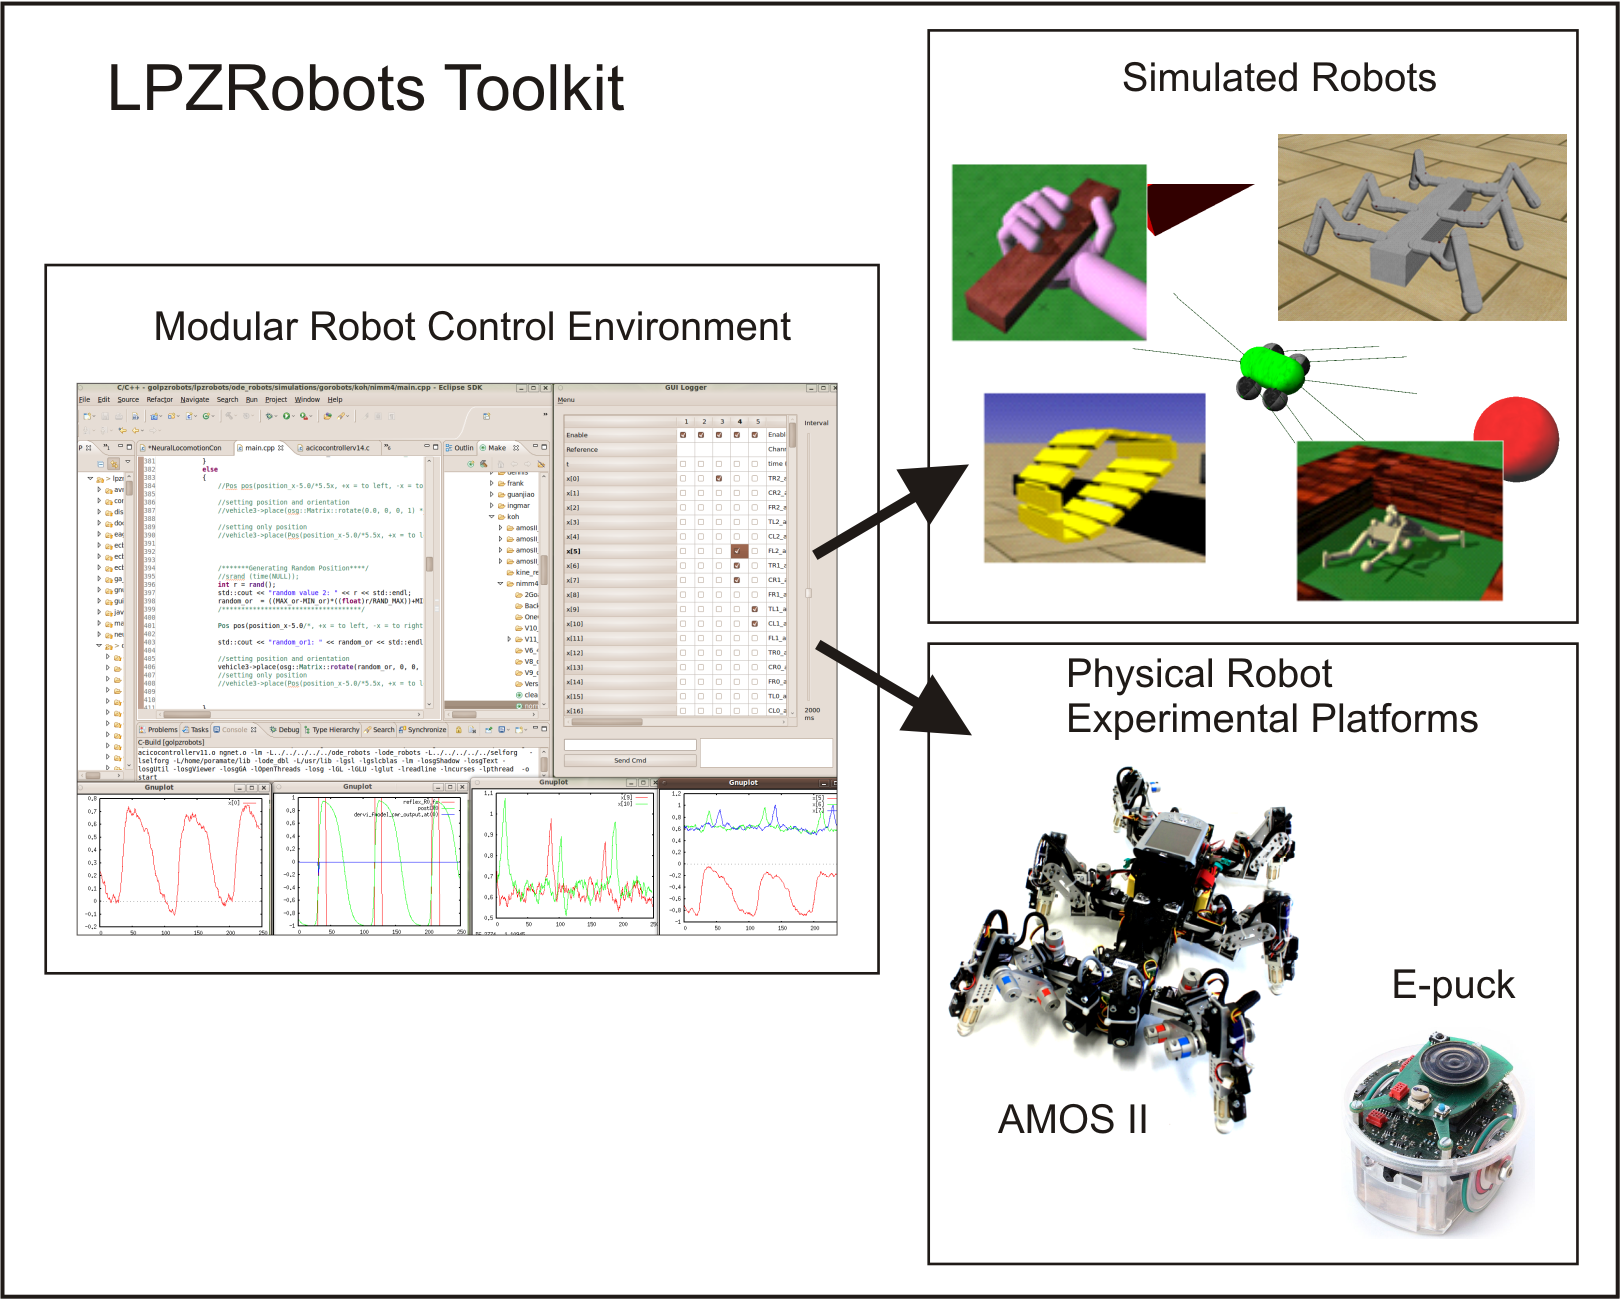
\includegraphics[width=8cm]{./Pics/AIdiagram.png}
\end{center}


\thispagestyle{empty}
\newpage
\thispagestyle{empty}
\tableofcontents


\newpage
\pagestyle{fancy} %eigener Seitenstil
\fancyhf{} %alle Kopf- und Fußzeilenfelder bereinigen
\fancyfoot[L]{\small{LpzRobots and GoRobotos Installation Manual}} %Kopfzeile links
\renewcommand{\headrulewidth}{0pt}
\fancyfoot[R]{\small{Page \small{\thepage} of \pageref*{LastPage}}} %Seitennummer


\section{Introduction}

The LpzRobots-Simulation is a robot simulation programmed at the university of Leipzig. Its main features
include the \emph{ode\_robots}, which is a 3D robot simulator, that is physically correct, and the so called
\emph{selforg}, that is a framework for controller implementation. \\
The important parts of the software architecture are shown in Figure: \ref{architecture}: \\
\begin{center}
\begin{figure}[h!]
 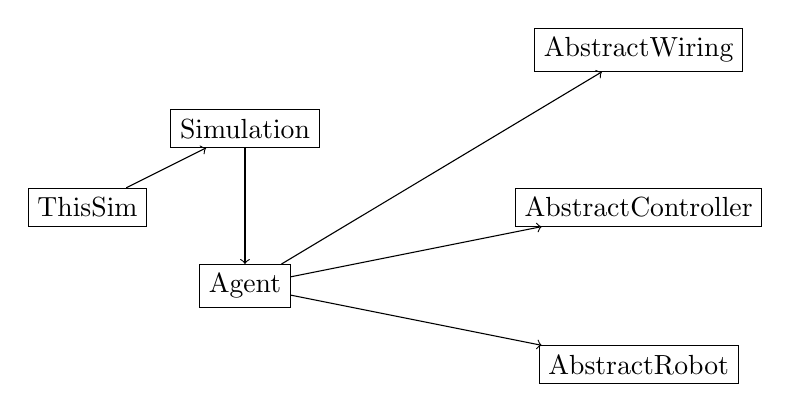
\begin{tikzpicture}
  \node at (0,2) (1) [rectangle,draw] {ThisSim};
  \node at (2,1) (2) [rectangle,draw] {Agent};
  \node at (2,3) (3) [rectangle,draw] {Simulation};
  \node at (7,0) (4) [rectangle,draw] {AbstractRobot};
  \node at (7,2) (5) [rectangle,draw] {AbstractController};
  \node at (7,4) (6) [rectangle,draw] {AbstractWiring};
  \path[->]
	      (3) edge (2)
	      (1) edge (3)
	      (2) edge (4)
	      (2) edge (5)
	      (2) edge (6)
	      ;
 \end{tikzpicture}
 \caption{Software Architecture for LpzRobots and GoRobotos}
 \label{architecture}
\end{figure}
\end{center}
\emph{ThisSim} will, during a simulation, integrate all elements of this very simulation, which means controlling
the environment, the robot, as well as setting initial parameters and plotting or logging data. \\
\emph{Agent} will integrate all elements of an agent by using the shown classes, one can for example add sensory preprocessing
using a child class of \emph{AbstractWiring}. \newline
\begin{center}
  \begin{figure}[h!]
     \begin{tikzpicture}{Simulation}
  \small
  \node at (0,4) (mainE) [rectangle,draw] {\emph{Simulated Environment}: main.cpp};
  \node at (0,6) (amos) [rectangle,draw] {\emph{Simulated Robot}: amonsII.cpp$\backslash$h};

  \node at (0,2) (mainR) [rectangle,draw] {\emph{Real Environment}: main.cpp};
  \node at (0,0) (real) [rectangle,draw] {\emph{Real Robot}: AMOSII\_serial.cpp$\backslash$h};

  \node at (6,5) (amosC) [rectangle,draw] {amosIIcontrol.cpp$\backslash$h};
  \node at (8.5,3.25) (NP) [rectangle,draw] {NeuralProcessing.ccp$\backslash$h};
  \node at (8.5,2.5) (NL) [rectangle,draw] {NeuralLocomotion.cpp$\backslash$h};
  \node at (9,1.5) (CPG) [] {CPG().cpp$\backslash$h};
  \node at (9,1) (PCPG) [] {POSTCPG().cpp$\backslash$h};
  \node at (9,0.5) (PSN) [] {PSN().cpp$\backslash$h};
  \node at (9,0) (VRN) [] {VRN().cpp$\backslash$h};
  \path[->]
	      %(mainE) edge (amos)
	      (mainE) edge (amosC)
	      (mainR) edge (amosC)
	      (mainR) edge (real)
	      (6,2.5) edge (NL)
	      (6,3.25) edge (NP)
	      (7,0) edge (VRN)
	      (7,0.5) edge (PSN)
	      (7,1) edge (PCPG)
	      (7,1.5) edge (CPG)
	      (mainE) edge (amos)
	      ;
  \path[-]
	      (amosC) edge (6,2.5)
	      (7,2.25) edge (7,0)
	      ;


\draw[dashed,color=blue] (-3, 3.5) to (3, 3.5);
\draw[dashed,color=blue] (3, 3.5) to (3, 6.5);
\draw[dashed,color=blue] (3, 6.5) to (-3, 6.5);
\draw[dashed,color=blue] (-3,6.5) to (-3, 3.5);

\draw[dashed,color=red] (-3, -0.5) to (3, -0.5);
\draw[dashed,color=red] (3, -0.5) to (3, 2.5);
\draw[dashed,color=red] (3, 2.5) to (-3, 2.5);
\draw[dashed,color=red] (-3,2.5) to (-3, -0.5);

\draw[dashed,color=mygreen] (4, -0.5) to (11, -0.5);
\draw[dashed,color=mygreen] (11, -0.5) to (11, 6.5);
\draw[dashed,color=mygreen] (11, 6.5) to (4, 6.5);
\draw[dashed,color=mygreen] (4,6.5) to (4, -0.5);
	      

\node at (1.75,1) (sim) [] {\emph{Reality}};
\node at (1.75,5) (reall) [] {\emph{Simulation}};
\node at (7.75,6) (reall) [] {\emph{Control}};
 \end{tikzpicture}
\caption{Need name for this picture}
  \end{figure}


\end{center}
\newpage
For working with the LpzRobots-Simulation, you will need a couple of things:
\begin{enumerate}
 \item A (preferably up-to-date) UNIX-based Operating System (state of the art: Ubuntu 11.10 or Debian 6.0)
 \item The Eclipse-Software combined with the following packages:
      \begin{itemize}
       \item C/C++ SDK
       \item The EGit-Tool-Kit
      \end{itemize}
 \item Access to the Assembla-Repository (contact your supervisor for access)
 \item The setUpGoRobots.zip file (contact your supervisor for the file)
\end{enumerate}
\section{Setting up Eclipse and LpzRobots}

\subsection{Running setUpGoRobots.sh}
% MENTION /HOME/YOURLOGIN ?????
From your supervisor, you will receive the .zip-File \emph{setUpGoRobots.zip} - or you can find it at \emph{gorobots/docs/install\_script/}. To begin with, you need to extract the files and the script \emph{setUpGoRobots.sh} within.
This script will:
\begin{enumerate}
 \item Install the required packages on your computer
 \item Include important settings to your \emph{.bashrc}
 \item Fetch the repositories \emph{LpzRobots} and \emph{GoRobots}
 \item Import the project settings file
 \item Compile the files
\end{enumerate}
Please note, that you need to be \emph{root} to install the packages via this script!.\\
After extracting, you can run the script, by typing \emph{./setUpGoRobots.sh} in the corresponding directory.

\subsubsection{Forking a repository}
The script will ask you for the URL of your forked repository. Please read about how to fork a network with Assembla in Section \ref{forksection}.

\subsection{Setting up Eclipse}

\subsubsection{Installing Tool-Kits within Eclipse} 
Before importing the repositories, you need two tool-kits for your Eclipse:
\begin{enumerate}
 \item To install a tool-kit, go to \emph{Help}$\rightarrow$\emph{Install Software}
 \item The first tool-kit you need is the C++ Development Kit. Work with the following link:\\ \url{http://download.eclipse.org/tools/cdt/releases/indigo} \\ and install the so called \emph{CDT}-Tool-kits.
 \item The second tool-kit is EGIT for accessing GIT within Eclipse. You can download it working with this link:\\ \url{http://download.eclipse.org/egit/updates}. Whilst doing so, you have to \emph{check} the box for \emph{Eclipse Git Team Provider} and \emph{uncheck} the box for \emph{EGit Mylyn}.
\end{enumerate}

\subsubsection{Importing the Repositories}

Once you have finished running the script and have installed the tool-kits, you are ready to import the repositories into your Eclipse. \\
To do so, first switch into the \emph{Git Repositories - View} within Eclipse. You can do this by clicking: \emph{Window}$\rightarrow$\emph{Show View}$\rightarrow$\emph{Other}$\rightarrow$\emph{Git}$\rightarrow$\emph{Git-Repositories} and hit \emph{OK}.
In this view, you can choose \emph{Add an existing local GIT repository}. The script will have placed the files at \emph{/home/yourlogin/workspace}.

\subsubsection{Code-Style withing Eclispe}
To adapt the Code-Style, go \emph{Window}$\rightarrow$\emph{Preferences}$\rightarrow$\emph{C/C++}$\rightarrow$ \\ \emph{Code-Style}$\rightarrow$\emph{Import}. Now you choose the file:\\ \nolinkurl{workspace/lpzrobots/codeStyleEclipse.xml} and hit \emph{apply}.

\subsection{Troubleshooting}

If you encounter any problems while using the script, please contact Frank or me (\emph{c.rauterberg@gmx.de}) and send us error output, solutions you found, etc. if possible. Find the install-by-hand-instructions at the end of this manual.
\section{Project Structure}

We use, as already mentioned, two GIT repositories, LpzRobots and GoRobots. A rough overview of the structure is given below in Figure \ref{struc}:


Later, the controllers for each robot will be implemented within \emph{GoRobots}, accessing the robots, which are located in \emph{LpzRobots}. The folder \emph{DEMO} will later contain demos of the different robots.
Another visualisation of the two repositories and where which file belongs is given in Figure \ref{struc2}. 
\begin{figure}[h!]
 \begin{center}
  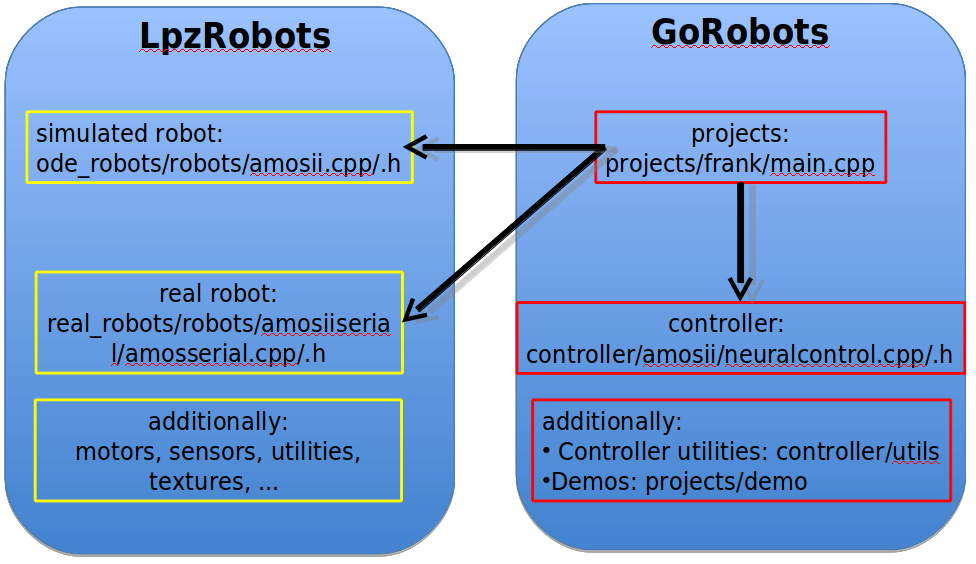
\includegraphics[width=10cm]{./Pics/struct.png}
 \end{center}
\caption{Structure of the two repositories, LpzRobots and GoRobots}
\label{struc2}
\end{figure}

You will later work with your own copy of the two repositories.

\newpage

\begin{figure}[h!]
 \begin{center}
  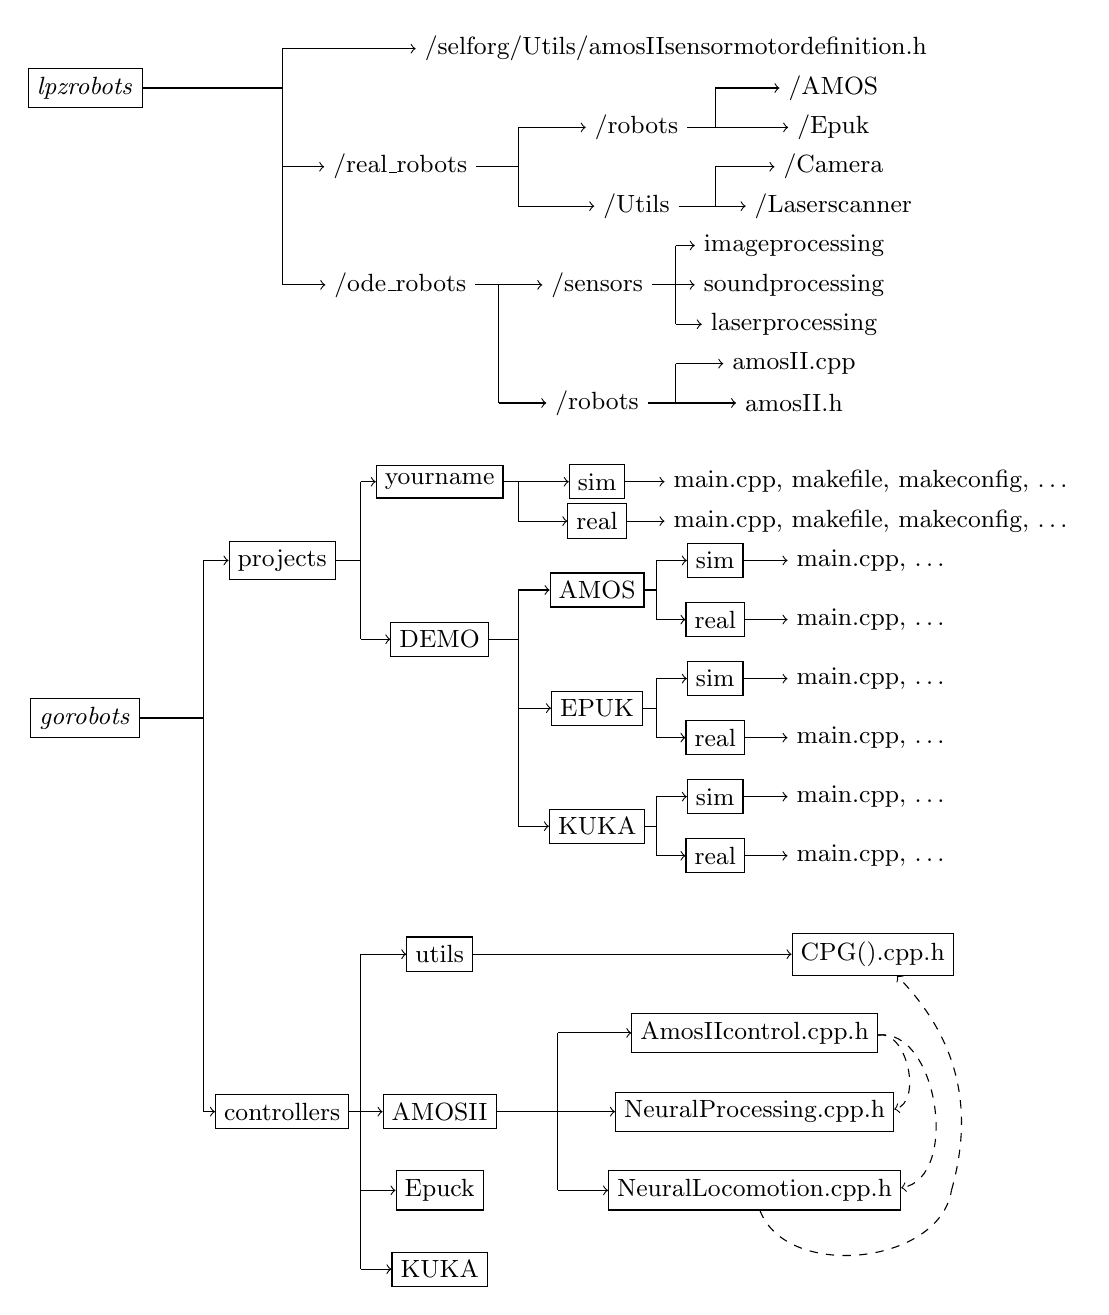
\begin{tikzpicture}{gitbranches}
   \small
  \node at (-1,-2) (lpz) [rectangle,draw] {\emph{lpzrobots}};
  \node at (3,-3) (realR) [] {/real\_robots};
  \node at (6.5,-1.5) (selforg) [] {/selforg/Utils/amosIIsensormotordefinition.h};
  \node at (3,-4.5) (odeR) [] {/ode\_robots};
  \node at (5.5,-4.5) (sensors) [] {/sensors};
  \node at (5.5,-6) (robots) [] {/robots};
  \node at (8,-4) (IP) [] {imageprocessing};
  \node at (8,-4.5) (SP) [] {soundprocessing};
  \node at (8,-5) (P) [] {laserprocessing};
  \node at (8,-5.5) (ACPP) [] {amosII.cpp};
  \node at (8,-6) (AH) [] {amosII.h};

\node at (6, -2.5) (RRrobots) [] {/robots};
\node at (6, -3.5) (RRutils) [] {/Utils};

\node at (8.5, -2) (RRamos) [] {/AMOS};
\node at (8.5, -2.5) (RRepuk) [] {/Epuk};

\node at (8.5, -3) (RRcamera) [] {/Camera};
\node at (8.5, -3.5) (RRlsc) [] {/Laserscanner};


   \path[->]
	      ( 1.5,-3) edge (realR)
	      ( 1.5,-1.5) edge (selforg)
	      ( 1.5,-4.5) edge (odeR)
	      (4.25,-4.5) edge (sensors)
	      (4.25,-6) edge (robots)
	      (6.5,-4) edge (IP)
	      (6.5,-4.5) edge (SP)
	      (6.5,-5) edge (P)
	      (6.5,-5.5) edge (ACPP)
	      (6.5,-6) edge (AH)
	      (4.5, -2.5) edge (RRrobots)
	      (4.5, -3.5) edge (RRutils)
	      (7, -2) edge (RRamos)
	      (7, -2.5) edge (RRepuk)
	      (7, -3) edge (RRcamera)
	      (7, -3.5) edge (RRlsc)
	      ;
  \path[-]
	      (lpz) edge ( 1.5,-2)
	      (1.5,-1.5) edge (1.5,-4.5)
	      (odeR) edge (4.25,-4.5)
	      (4.25,-4.5) edge (4.25, -6)
	      (sensors) edge (6.5,-4.5)
	      (robots) edge (6.5,-6)
	      (6.5,-4) edge (6.5,-5)
	      (6.5, -5.5) edge (6.5,-6)
	      (realR) edge (4.5,-3)
	      (4.5, -2.5) edge ( 4.5, -3.5)
	      (RRrobots) edge (7, -2.5)
	      (7, -2) edge (7, -2.5)
	      (RRutils) edge (7, -3.5)
	      (7, -3) edge (7, -3.5)
	      ;


   \node at (-1,-10) (gorobots) [rectangle,draw] {\emph{gorobots}};
   \node at (1.5,-8) (projects) [rectangle,draw] {projects};
   \node at (1.5,-15) (controllers) [rectangle,draw] {controllers};
   \node at (3.5,-7) (yn) [rectangle,draw] {yourname};
   \node at (3.5,-9) (demo) [rectangle,draw] {DEMO};
   \node at (5.5,-7) (sim) [rectangle,draw] {sim};
   \node at (5.5,-7.5) (real) [rectangle,draw] {real};

   \node at (9,-7) (simS) [] {main.cpp, makefile, makeconfig, \ldots};
   \node at (9,-7.5) (realS) [] {main.cpp, makefile, makeconfig, \ldots};
   
    \node at (5.5, -8.375) (AMOS) [draw] {AMOS};
    \node at (5.5, -9.875) (EPUK) [draw] {EPUK};    
    \node at (5.5, -11.375) (KUKA) [draw] {KUKA};

    \node at (7,-8) (AMOSsim) [draw] {sim};
    \node at (9,-8) (AMOSsimS) [] {main.cpp, \ldots};
    \node at (7,-8.75) (AMOSreal) [draw] {real};
    \node at (9,-8.75) (AMOSrealS) [] {main.cpp, \ldots};
    \node at (7,-9.5) (EPUKsim) [draw] {sim};
    \node at (9,-9.5) (EPUKsimS) [] {main.cpp, \ldots};
    \node at (7,-10.25) (EPUKreal) [draw] {real};
    \node at (9,-10.25) (EPUKrealS) [] {main.cpp, \ldots};
    \node at (7,-11) (KUKAsim) [draw] {sim};
    \node at (9,-11) (KUKAsimS) [] {main.cpp, \ldots};
    \node at (7,-11.75) (KUKAreal) [draw] {real};
    \node at (9,-11.75) (KUKArealS) [] {main.cpp, \ldots};

    \node at (3.5,-13) (utils) [draw] {utils};
    \node at (3.5,-15) (AMOSII) [draw] {AMOSII};
    \node at (9,-13) (AMOSCPG) [draw] {CPG().cpp.h};
    \node at (3.5,-16) (EPUKCon) [draw] {Epuck};
    \node at (3.5,-17) (KUKACon) [draw] {KUKA};


    \node at (7.5,-14) (AMOSIICon) [draw] {AmosIIcontrol.cpp.h};
    \node at (7.5,-15) (AMOSIINP) [draw] {NeuralProcessing.cpp.h};
    \node at (7.5,-16) (AMOSIINL) [draw] {NeuralLocomotion.cpp.h};

\draw[dashed,bend left=89, ->] (AMOSIICon) to (AMOSIINP);
\draw[dashed,bend left=89, ->] (AMOSIICon) to (AMOSIINL);


   \path[->]
    (0.5,-8) edge (projects)
    (0.5,-15) edge (controllers)
    (2.5,-7) edge (yn)
    (2.5, -9) edge (demo)
    (4.5,-7) edge (sim)
    (4.5,-7.5) edge (real)
    (sim) edge (simS)
    (real) edge (realS)
    (4.5, -8.375) edge (AMOS)
    (4.5, -9.875) edge (EPUK)
    (4.5, -11.375) edge (KUKA)
    (6.25, -8) edge (AMOSsim)
    (6.25, -8.75) edge (AMOSreal)
    (6.25, -9.5) edge (EPUKsim)
    (6.25, -10.25) edge (EPUKreal)
    (6.25, -11) edge (KUKAsim)
    (6.25, -11.75) edge (KUKAreal)
    (AMOSsim) edge (AMOSsimS)
    (AMOSreal) edge (AMOSrealS)
    (EPUKsim) edge (EPUKsimS)
    (EPUKreal) edge (EPUKrealS)
    (KUKAsim) edge (KUKAsimS)
    (KUKAreal) edge (KUKArealS)
    (utils) edge (AMOSCPG)
    (2.5,-13) edge (utils)
    (2.5,-15) edge (AMOSII)
    (2.5, -16) edge (EPUKCon)
    (2.5,-17) edge (KUKACon)
    (5,-14) edge (AMOSIICon)
    (5,-15) edge (AMOSIINP)
    (5,-16) edge (AMOSIINL)
    ;

   \path[-]
    (gorobots) edge (0.5,-10)
    (0.5,-8) edge (0.5,-15)
    (projects) edge ( 2.5,-8)
    (2.5, -7) edge (2.5, -9)
    (yn) edge (4.5, -7)
    (4.5,-7) edge (4.5,-7.5)
    (demo) edge (4.5,-9)
    (4.5, -8.375) edge (4.5,-11.375)
    (AMOS) edge (6.25,-8.375)
    (EPUK) edge (6.25,-9.875)
    (KUKA) edge (6.25,-11.375)
    (6.25,-8) edge (6.25,-8.75)
    (6.25,-9.5) edge (6.25,-10.25)
    (6.25,-11) edge (6.25,-11.75)
    (controllers) edge (2.5,-15)
    (2.5,-13) edge (2.5,-17)
    (AMOSII) edge (5,-15)
    (5,-14) edge (5,-16)
    
    ;
\draw[dashed,bend right=75] (AMOSIINL) to (10,-16);
\draw[dashed, ->, bend right] (10,-16) to (AMOSCPG);

% \draw (AMOSIINL) to [bend right] (AMOSCPG) node {};


\end{tikzpicture}
 \end{center}
\caption{Structure of the two repositories, LpzRobots and GoRobots}
\label{struc}
\end{figure}
\section{Working with GIT}

\subsection{Overview of GIT-commands}

The following picture will give a good overview over the workflow and the commands in GIT:\\
\begin{figure}[h!]
 \begin{center}
  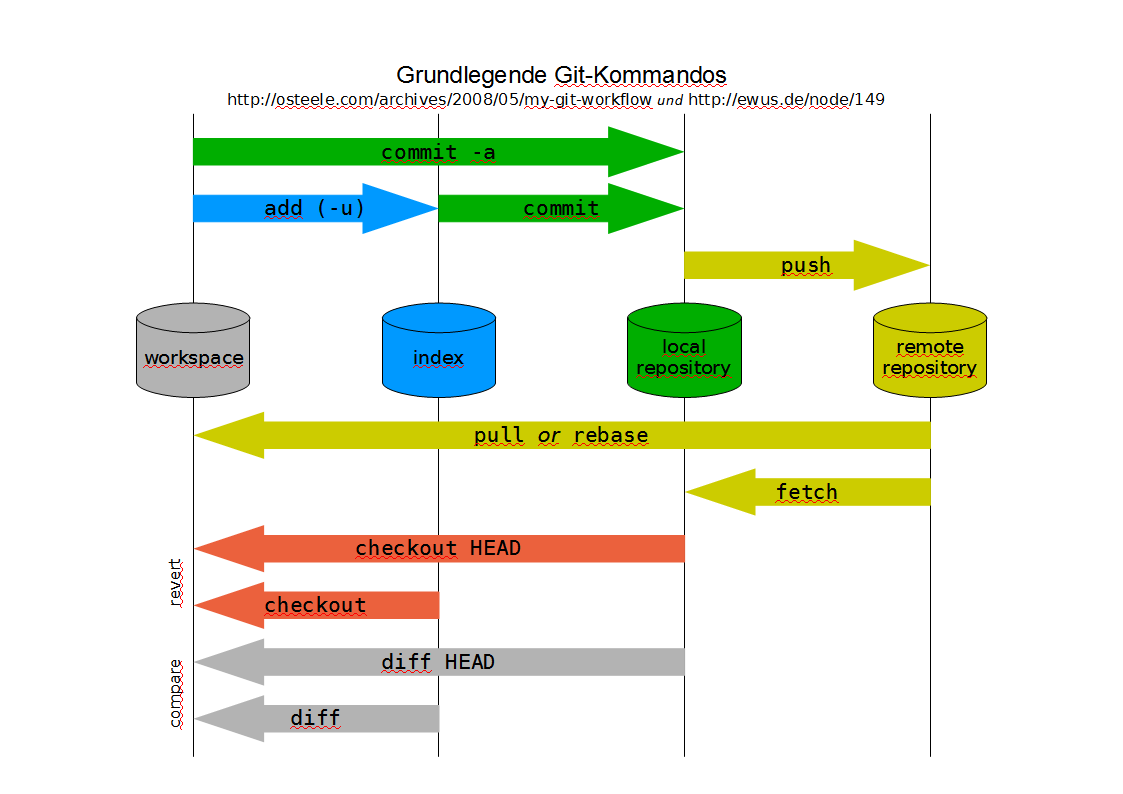
\includegraphics[width=12cm,height=9cm]{./pics/git.png}
 \end{center}
 \caption{An Overview over GIT commands}
\end{figure}
The main advantage in GIT is, that every host has got his own local repository, which in itself is an external repository to another host.\newpage 
I will give an example, in which I will try, to use most of the commands GIT gives us:
\begin{itemize}
 \item You create a new file in your workspace in your own branch, that was not under version control before
 \item Now you first have to add it to the \emph{index}, which for GIT is just a list of files, that it has to monitor. You can do this using \emph{add}
 \item The next step is adding the actual file to the local repository. You can do this via \emph{commit}
 \item Now the file is under version control. You can now could get the file from the repository using \emph{checkout HEAD}
 \item If you also want to add the file to the remote repository, you can use \emph{push}
 \item Now another person can get your whole work using \emph{pull}, which will provide him with everything, that is currently listed in your \emph{remote repository}
\end{itemize}
\remph{Please note: Be careful whilst merging, Eclipse will offer you to ``overwrite'', which is not a good idea, as it does exactly what it promisses instead of merging. We will support this warning with a screenshot if possible!}
To provide a full overview over the commands, I will list all the commands, that Eduard did show us in his presentation:
\begin{itemize}
 \item \emph{git add}: adds file changes in your workspace to your index
 \item \emph{git commit}: Commits all the changes listed in the index to the local repository
 \item \emph{git push}: Pushes local branch to the remote repository
 \item \emph{git fetch}: Fetches all files from the remote repository, that are not in the local repository
 \item \emph{git merge}: Merges one or more branches into your current branch
 \item \emph{git pull}: Fetches files from remote repository and merges them with local files (equal to \emph{git fetch; git merge})
 \item \emph{git rm}: Removes a file from your repository 
\end{itemize}
\newpage
\subsection{Setting up your own branch with GIT}
Within your repository, you should still create branches for each feature you develop.
To create a new branch you simple do:
\begin{enumerate}
 \item In Eclipse, right-click on \emph{name\_of\_your\_fork}
 \item Select \emph{Team}$\rightarrow$\emph{Switch to}$\rightarrow$\emph{New Branch} 
 \item As shown in the picture bellow, select the source:\\ \emph{refs/remotes/origin/goettingen\_master}\footnote{By choosing this, you make sure, that you have the latest online version} 
% Hier nachfragen, wie das ganze jetzt ist, mit MASTER und GOETTINGEN_MASTER  
 \item Choose a name following the scheme yourname\_yourfeature
 \item Activate the checkbox for checking out the new branch
 \item Work away
\end{enumerate}

\begin{figure}[h!]
 \begin{center}
 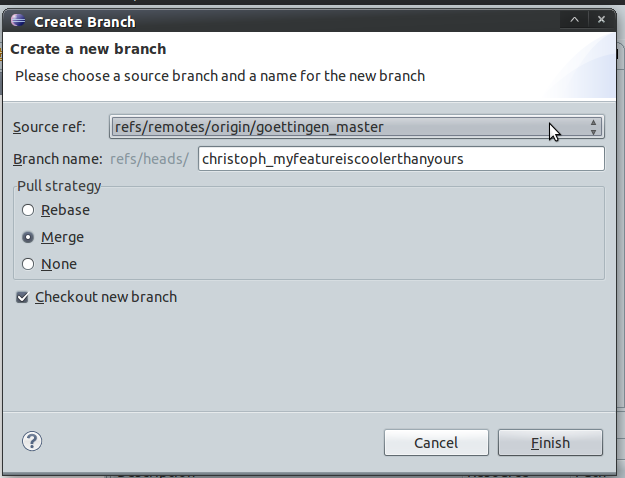
\includegraphics[height=8cm]{./pics/NewBranchSmall.png}
\end{center}
\caption{How to create a new branch within Eclipse}
\end{figure}



\newpage

\subsection{Forking a Repository}
\label{forksection}
To create a fork of a repository, you need access to the assembla-website. Once you have logged in, you can choose a repository and then click on the button \emph{fork network}.
One click on the button \emph{fork} will then create a fork of the repository for you, as shown in Figure \ref{fork}. You will furthermore be asked for a name of this copy of the repository, remember this name, as you will need it for the setup!

\begin{figure}[h!]
\begin{center}
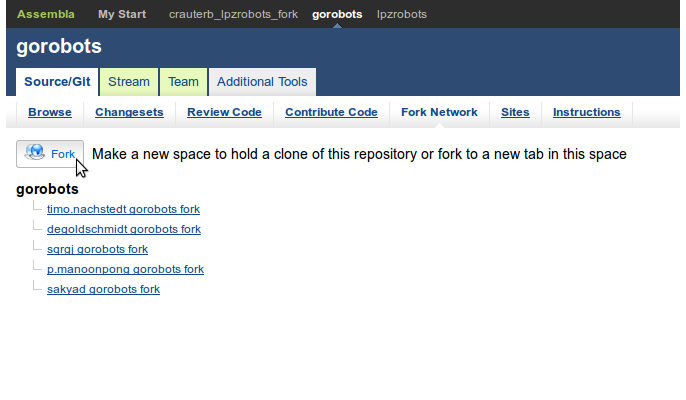
\includegraphics[width=12cm]{./pics/Fork.png}
\caption{How to fork a repository at the Assembla website}
\label{fork}
\end{center}
\end{figure}

\subsection{Merging}
Please check with your supervisor, before merging back into \emph{master}. \\
If you want to merge a branch of yours, you will have to send a merge request via the assembla-webpage. A supervisor will then have a look at your code. \emph{BUT} he is only able to do so,
if you have given him or her the rights to read your code. You can do so by, on the assembla-webpage in your forked repository, select \emph{team} and then, on the right, select \emph{Invite people from other teams}.
No you can choose which one you want to invite, and then you can choose which rights you want to give him or her.

\subsection{How to update your Master Branch}

Make sure that you are in your master branch by typing:
\begin{lstlisting}
~/workspace/YOURLOGIN-gorobots-fork $ git branch
\end{lstlisting}
The output should be something like this:
\begin{lstlisting}
  goplus
  feature_branch_1
  feature_branch_2
  feature_branch_3
* master 
\end{lstlisting}
The star indicates, in which branch you are working right now. If you are not working in the \emph{master}-branch, switch to the branch by typing:
\begin{lstlisting}
 ~/workspace/YOURLOGIN-gorobots-fork $ git checkout master
\end{lstlisting}
You can use \emph{git branch} again, to check of you are in the right branch now.

If you are in the master branch type
\begin{lstlisting}
~/workspace/YOURLOGIN-gorobots-fork$ git remote -v
\end{lstlisting}
The output should be something like this (if you did not add a remote before):
\begin{lstlisting}
origin https://YOURLOGIN@git.assembla.com/YOURLOGIN-gorobots-fork.git (fetch)
origin https://YOURLOGIN@git.assembla.com/YOURLOGIN-gorobots-fork.git (push)
\end{lstlisting}
Now you have to add a stable repository as additional remote type:
\begin{lstlisting}
git remote add stable https://YOURLOGIN@git.assembla.com/gorobots.git 
\end{lstlisting}
\emph{git remote -v} should now show something like:
\begin{lstlisting}
~/workspace/YOURLOGIN-gorobots-fork $ git remote -v
origin https://YOURLOGIN@git.assembla.com/YOURLOGIN-gorobots-fork.git (fetch)
origin https://YOURLOGIN@git.assembla.com/YOURLOGIN-gorobots-fork.git (push)
stable https://YOURLOGIN@git.assembla.com/gorobots.git (fetch)
stable https://YOURLOGIN@git.assembla.com/gorobots.git (push) 
\end{lstlisting}
This means you are able to connect to the stable repository (referred to as stable) from your local repository. \\
Now update your local repositories information about the stable repository by typing:
\begin{lstlisting}
~/workspace/YOURLOGIN-gorobots-fork $ git fetch stable  
\end{lstlisting}
After typing your password you see an output like the following:
\begin{lstlisting}
From https://git.assembla.com/gorobots
 * [new branch]      master     -> stable/master 
\end{lstlisting}
Your local repository knows now what branches are available in the stable repository.\\
Now merge the changes of the stable master in your workspace (which currently contains your local master branch) by typing:
\begin{lstlisting}
~/workspace/YOURLOGIN-gorobots-fork $ git merge stable/master 
\end{lstlisting}
If there were now changes, the Output would be something like:
\begin{lstlisting}
Already up-to-date. 
\end{lstlisting}
An example of an output including changes would look like:
\begin{lstlisting}
Updating 1054d9a..330d652
Fast-forward
 docs/README                |    6 ++++++
 docs/install_manual/README |    5 +++++
 docs/install_script/README |    6 ++++++
 3 files changed, 17 insertions(+), 0 deletions(-)
 create mode 100644 docs/README
 create mode 100644 docs/install_manual/README
 create mode 100644 docs/install_script/README 
\end{lstlisting}
Now you can use \emph{git commit}, to commit changes to your local repository, and \emph{git push}, to commit changes to the remote repository. \\
Now your master branch is up to date with our stable version and you can continue with the next section.


\section{Installing LpzRobots by Hand}


% HIER MUSS NOCH DER PFAD HIN !!!!!!!!!!!
% Es wuerde sich anbieten, das Skript genau da hin zu schmeißen, wo auch die Readme in GoMasters ist
Before you install LpzRobots, you first need to install a couple of additional packages. You can do this using the following commands:\\
% SUBVERSION IS STILL LISTED HERE - DO WE STILL NEED THIS??????
% \emph{sudo apt-get install g++ make m4 libreadline-dev libgsl0-dev libglu-dev $\backslash$ \\ libgl1-mesa-dev libopenscenegraph-dev libqt4-dev qt4-qmake libqt4-qt3support$\backslash$ \\ openjdk-6-jdk automake gnuplot libgsl0ldbl xutils-dev libltdl-dev $\backslash$ \\ libtool subversion eclipse-platform eclipse-pde} \\
\emph{sudo apt-get install$\backslash$ \\
 g++  make  automake libtool xutils-dev m4  libreadline-dev  libgsl0-dev$\backslash$ \\
 libglu-dev libgl1-mesa-dev freeglut3-dev  libopenscenegraph-dev$\backslash$ \\
 libqt4-dev libqt4-opengl libqt4-opengl-dev qt4-qmake  libqt4-qt3support gnuplot}\footnote{You can also find this list of dependencies in the repository \emph{lpzrobots}}\\
Also, you will need this package: \\
% \emph{sudo apt-get install freeglut3 freeglut3-dev} \\
\emph{sudo apt-get install binutils-gold}\footnote{You may need this only for newer Ubuntu-Versions ($>=11.10$), as the linker does not link anymore} \\
Furthermore, you will need to add some lines to your \emph{.bashrc}: \\
\small{
\begin{tabbing}
\# definitions for lpzrobots \\
   export CPATH="\$HOME$/$include"\\
  export LIBRARY\_PATH="\$HOME$/$lib"\\
  export LD\_LIBRARY\_PATH=\$\{LD\_LIBRARY\_PATH\}:\$HOME$/$lib:$/$usr$/$lib$/$osgPlugins2.8.1\\
  export PATH=\$\{PATH\}:\$HOME$/$bin\\
\end{tabbing}}
Now you are ready to install the LpzRobot-Simulation. \\
As Eclipse has now synchronized its workspace with the GIT-Repository, you can find the setup-files in your workspace.\\ To install LpzRobots, go to \emph{workspace}$\rightarrow$\emph{lpzrobots}
and run make (all). \\
Install it to \emph{/home/YOURLOGIN} and choose \emph{install as developer},\\ which is the shortcut \emph{d}
\section{FAQs}

\subsection{Installation errors in general}

\subsubsection{Symbol lookup error}
After installing the "binutils-gold" package, I get the following error after recompiling my source code:
"./test: symbol lookup error: /usr/local/lib/liburg.so.0: undefined symbol: \_ZTIN3qrk10CoordinateE"
(Note: liburg is a library for the Hokuyo laser scanners from here or via packet manager).\\

As "binutils-gold" contains a different linker for C++ files, which is optimized for speed, it is likely that this new linker does not link the laser scanner libraries correctly (probably due to "bad" programming within the drivers).
However, this new linker is not necessary for compiling and running lpzrobots, it just speeds up the compilation time.
So the solution to the problem is simple: Uninstall "binutils-gold" and everything works.


\subsection{Errors using setUpGoRotobots.sh}

\subsubsection{Error with \emph{git clone}}

Whilst cloning the repositories, I encountered the following error:
\begin{lstlisting}
git clone https://crauterb@git.assembla.com/lpzrobots.git -b master
Cloning into crauterb-lpzrobots-fork...
Password:
remote: Counting objects: 25478, done.
remote: Compressing objects: 100% (6030/6030), done.
remote: Total 25478 (delta 19211), reused 25478 (delta 19211)
Receiving objects: 100% (25478/25478), 19.97 MiB | 527 KiB/s, done.
Resolving deltas: 100% (19211/19211), done.
warning: Remote branch master not found in upstream origin, using HEAD instead
warning: remote HEAD refers to nonexistent ref, unable to checkout.
\end{lstlisting}

the repository Lpzrobots when there was no branch \emph{master}, and for some reason, it was not added later and did not appear anywear.
The solution was simple: Delete the forked version and create a new one - if possible. Worked for me.



\subsection{Problems with GIT}

\subsubsection{Setting up Repositories in Eclipse}
\label{EclipseGIT}
In some cases, the instructions on how to set up the GIT-repositories within Eclipse did not work. \\
Here is a different approach, that worked for me: \\
\begin{enumerate}
 \item Import the repositories into the GIT-view of Eclipse, just as described before
 \item Instead of importing over the GIT-View, you now go onto \emph{File $\rightarrow$ Import $\rightarrow$ General $\rightarrow$ Existing Projects into Workspace} and you then choose the two repositories
 \item After Eclipse has imported the files, you can \emph{right-click} on the Project, and then select \emph{Team $\rightarrow$ Share}
 \item Now, just select \emph{GIT} and the two GIT-repository-adresses should appear
 \item \emph{Apply}
\end{enumerate}


\subsubsection{No Connection to GIT Server: The remote end hung up unexpectedly.}

If you defined stable as usual (check with{\tt git remote -v}):\\
 \nolinkurl{stable}    \nolinkurl{https://wbj@git.assembla.com/lpzrobots.git (fetch)}\\
 \nolinkurl{stable}    \nolinkurl{https://wbj@git.assembla.com/lpzrobots.git (push)}\\\\
%
but when typing {\tt git fetch origin} you get the following error message: \\
{\tt Password for 'https://wbj@git.assembla.com':} \\
{\tt error: RPC failed; result=22, HTTP code = 401} \\
{\tt fatal: The remote end hung up unexpectedly} \\\\
%
and also defining the origin with http only:\\
\nolinkurl{stable_http}    \nolinkurl{http://wbj@git.assembla.com/lpzrobots.git (fetch)}\\
does not help, try to use the git protocol:\\
\nolinkurl{stable_git2}    \nolinkurl{git@git.assembla.com:lpzrobots.git (fetch)}\\
\nolinkurl{stable_git2}      \nolinkurl{git@git.assembla.com:lpzrobots.git (push)}










\subsection{Errors when starting the simulation}

The error messages was:

\begin{lstlisting}
> ./start
> ./start: error while loading shared libraries: libode\_dbl.so.1:
  cannot open shared object file: No such file or directory
\end{lstlisting}
The solution was:
\begin{lstlisting}
 > source ~/.bashrc
\end{lstlisting}


\begin{lstlisting}
if you use Ubuntu version 12.4 LTS, you might see this problem:

> ./start
> ./start: symbol lookup error: /usr/lib/libgsl.so.0: undefined symbol: cblas_dnrm2
\end{lstlisting}
The solution was:
\begin{lstlisting}
 > sudo apt-get remove binutils-gold
\end{lstlisting}



\subsection{Using Lpzrobots}
\begin{lstlisting}
> after start simulation , press 1 to fixed camera view
> Ctrl r = record movie
> .\start -f = record log file
> .\start = start program
> .\start -g 1 = display GUI
\end{lstlisting} 


\end{document}
